\subsubsectionwithauthor[author={Mika Landeck},email={mika.landeck@fau.de}]{Aufgabe 1: Reguläre Sprachen}
\paragraph{(a)}
	$L_a = \{w \in \Sigma^* | \nexists u,u' \in \Sigma^*: w =u(ab)u'\} = ((b|c)^*(a^*c)^*(b|c)^*)^*a^*$
	
	\textbf{Erklärung}: \\
	Alle Wörter in $L_a$ setzen sich aus Teilworten zusammen, die eine zusammenhängendes Teilwort beliebiger Länge aus $a$'s enthalten. Vor und nach dem $a$-Block dürfen beliebige Wörter aus $b$'s und $c$'s vorkommen (deshalb $(b|c)^*$ in regulären Ausdruck). Sobald ein $a$ erscheint, dürfen weitere $a$'s folgen (deshalb $a^*$ in regulären Ausdruck) oder ein $c$ (deshalb folgt auf $a^*$ immer das $c$, außer am Ende des Wortes). Es müssen auch gar keine $a$'s vorkommen (dehalb sind alle Bestandteile, in denen $a$'s vorkommen, mit $^*$ versehen).

\paragraph{(b)}
	$L_b = L(M) = a^*|(a^* ba^* ba^* ba^* ba^*)^*$.
	
	\textbf{Begründung}: \\
	Anfangs befinden wir uns in einem Endzustand, der beliebig viele weitere $a$'s zulässt (deshalb $a^*$ in regulären Ausdruck).\\
	Verlässt man diesen Endzustand über ein $b$, muss ein Zyklus mit genau vier $b$'s durchlaufen werden, zwischen denen jeweils beliebig viele $a$'s liegen dürfen, bevor wieder der Endzustand erreicht wird (deshalb $a^* ba^* ba^* ba^* ba^*$ in regulären Ausdruck). Dieser Zyklus kann beliebig oft durchlaufen werden (deshalb das $^*$ bei der rechten Klammer im regulären Ausdruck).
	
\paragraph{(c)}
	Zur besseren Übersicht wird zunächst die \textbf{Zustandsübergangs-Tabelle} des Automaten aufgestellt:\\
	\begin{tabular}{|c|c|c|}
		\hline
		\textbf{Zustand} & \textbf{0} & \textbf{1} \\
		\hline
		0                & 1          & 3 \\
		\hline
		1                & 0          & 6 \\
		\hline
		2                & 1          & 4 \\
		\hline
		3                & 4          & 4 \\
		\hline
		4                & 4          & 5 \\
		\hline
		5                & 0          & 5 \\
		\hline
		6                & 0          & 5 \\
		\hline
	\end{tabular} 
	
	Um die Erreichbarkeit aller Zustände zu überprüfen wird eine \textbf{Zeugentabelle} angefertigt:\\
	\begin{tabular}{l|ccccccc}
		\textbf{Zustand} & 0          & 1 & 2 & 3 & 4  & 5   & 6 \\
		\hline
		\textbf{Zeuge}   & $\epsilon$ & 0 & - & 1 & 11 & 111 & 01 \\
	\end{tabular} 
	Zustand 2 ist also nicht erreichbar, deshalb entfällt er im minimierten Automaten.
	
	Nun wird das bekannte \textbf{Tabellenfüllverfahren} zur Bestimmung äquivalenter Zustände durchgeführt: 
	
	\includegraphics[scale=0.7]{Tabellenfüllverfahren.png}

	Da Zusatnd 4 der einzige Endzustand ist, werden zunächst alle Zustandspaare in der Tabelle, die 4 und einen weiteren Zustand enthalten, mit $X_0$ markiert.
	
	Die weiteren Markierungen in der Tabelle gehen aus folgender Tabelle hervor, welche die Übergänge der Zustandspaare angibt:

	\begin{tabular}{c|c|c|l}
		\textbf{Zustandspaar} & \textbf{0} & \textbf{1} & \textbf{Erläuterung} \\
		\hline
		(0,1)                 & (0,1)      & (3,6)      & Eingabe 1: (3,6) führt zu X3. Ergänze X5. \\		
		\hline
		(0,3)                 & (1,4)      & (3,4)      & Eingabe 0: (1,4) führt zu X0. Ergänze X1. \\
		\hline
		(1,3)                 & (0,4)      & (4,6)      & Eingabe 0: (0,4) führt zu X0. Ergänze X4. \\
		\hline 		 		
		(0,5)                 & (0,1)      & (3,5)      & Eingabe 0: (3,5) führt zu X2. Ergänze X6. \\
		\hline 		
		(1,5)                 & (0,0)      & (5,6)      & \\
		\hline
		(3,5)                 & (0,4)      & (4,5)      & Eingabe 0: (0,4) führt zu X0. Ergänze X2. \\
		\hline
		(0,6)                 & (0,1)      & (3,5)      & Eingabe 1: (3,5) führt zu X2. Ergänze X7. \\
		\hline
		(1,6)                 & (0,0)      & (5,6)      & \\
		\hline
		(3,6)                 & (0,4)      & (4,5)      & Eingabe 0: (0,4) führt zu X0. Ergänze X3. \\
		\hline
		(6,5)                 & (0,0)      & (5,5)      & \\
	\end{tabular} 
	
	Die Zuständspaare 1, 5 und 6 bleiben nach wiederholtem Durchlaufen und Überprüfen unmarkiert. Folglich liegen 1, 5 und 6 in der selben Äquivalentsklasse und bilden im minimietern Automaten den Zustand $[1,5,6]$. Insgesamt ergeben sich also folgende Äquivalenzklassen als Zustände für den minimierten Automaten: $[0],[1,5,6],[3],[4]$
	
	Der minimierte Automat $A'$ sieht also folgendermaßen aus: \\
	$A' = (\{[0],[1,5,6],[3],[4] \},\{0,1\},\delta, [0], \{[4]\})$

	\begin{figure}[ht]
		\begin{minipage}[t]{.4\textwidth}
			\hspace*{25pt}
			mit $\delta$:

			\hspace*{25pt}
			\begin{tabular}{|l|l|l|}
				\hline
				\textbf{Zustand} & \textbf{0} & \textbf{1} \\
				\hline
				[0]            & [1,5,6]    & [3] \\ 
				\hline
				[1,5,6]        & [0]        & [1,5,6] \\
				\hline
				[3]            & [4]        & [4] \\
				\hline  
				[4]            & [4]        & [1,5,6] \\
				\hline 
			\end{tabular}
		\end{minipage}
		\begin{minipage}[t]{.57\textwidth}
			\vspace*{0pt}
			\hspace*{20pt}
			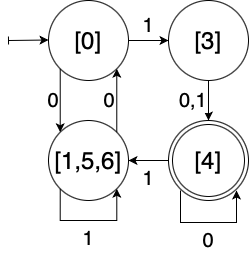
\includegraphics[scale=0.35]{DEA_T1_A1.png}
		\end{minipage} 
	\end{figure}
	